\documentclass{standalone}
\usepackage{tikz}
\usetikzlibrary{calc}

\begin{document}

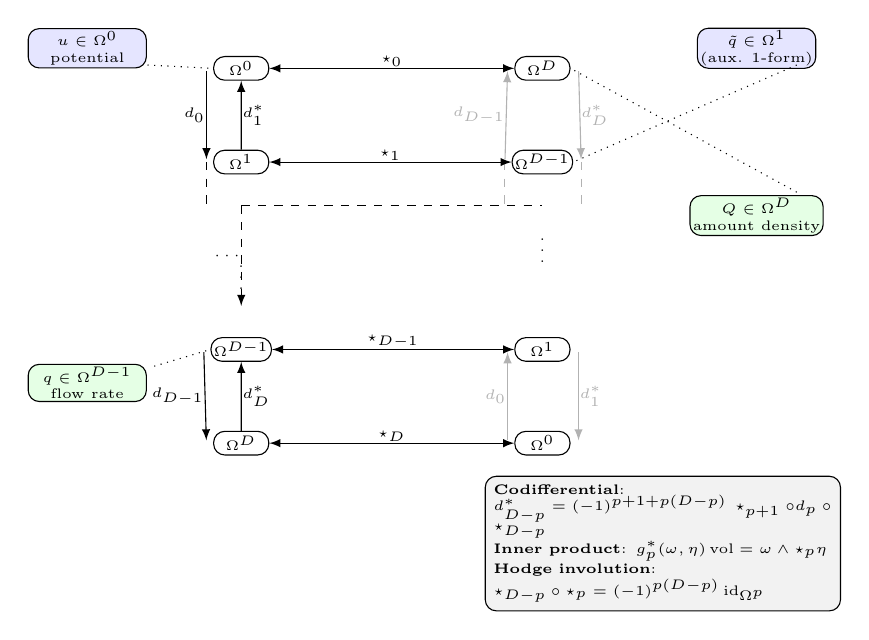
\begin{tikzpicture}[
    scale=0.85, % OVERALL SCALE: increase to enlarge entire diagram
    >=latex,
    % Box style: adjust inner sep, minimum width/height, font size
    box/.style={draw,rounded corners,align=center,fill=#1!10,inner sep=1pt,minimum width=0.7cm,minimum height=0.3cm,font=\tiny},
    % Label style: adjust font size
    lbl/.style={font=\tiny,inner sep=0.3pt}
]

% ==============================
% TUNING KNOBS - EDIT THESE TO ADJUST POSITIONS
% ==============================
\def\xL{-2.7}   % LEFT COLUMN x-position (move left: decrease, move right: increase)
\def\xR{1.8}    % RIGHT COLUMN x-position (spacing between columns = xR - xL)
\def\yTop{4.2}  % TOP ROW y-position (move up: increase, move down: decrease)
\def\dy{1.4}    % VERTICAL SPACING between rows (increase for more space)

% CORNER BOXES POSITIONS
\def\xLT{-5.0}  % TOP-LEFT corner x (potential u)
\def\yLT{4.5}   % TOP-LEFT corner y
\def\xLB{-5.0}  % BOTTOM-LEFT corner x (flow rate q)
\def\yLB{-0.5}  % BOTTOM-LEFT corner y
\def\xRT{7.5}   % TOP-RIGHT corner x (aux 1-form)
\def\yRT{4.5}   % TOP-RIGHT corner y
\def\xRB{7.5}   % BOTTOM-RIGHT corner x (amount Q)
\def\yRB{-0.5}  % BOTTOM-RIGHT corner y

% ==============================
% LEFT COLUMN: Ω^p (p=0 to D)
% ==============================
% Each node: adjust minimum width/height in box style, or add locally
\node[box=white] (L0)  at (\xL,\yTop-0*\dy) {$\Omega^{0}$};
\node[box=white] (L1)  at (\xL,\yTop-1*\dy) {$\Omega^{1}$};

\node[lbl]      (Ld1) at (\xL, \yTop-2*\dy - 0.2) {$\vdots$}; % Adjust yshift (0.2) to move dots
\node[box=white] (LDm) at (\xL,\yTop-3*\dy) {$\Omega^{D-1}$};
\node[box=white] (LD)  at (\xL,\yTop-4*\dy) {$\Omega^{D}$};

% UPWARD d_p ARROWS (exterior derivative) – slightly shifted left and shortened
\draw[->,shorten >=1pt, shorten <=1pt] ([xshift=-0.10cm]L0.west) -- node[lbl,left] {$d_0$} ([xshift=-0.10cm]L1.west);

% \draw[->,shorten >=1pt, shorten <=1pt] ([xshift=-0.10cm]L1.west) -- node[lbl,sloped,above,yshift=0.5pt] {$d_1$} +([xshift = -0.10cm]0,-0.95) coordinate (tmpd);

\draw[dashed] ([xshift=-0.10cm]L1.west) -- ++(0,-0.65); % Dashed middle section

\draw[->,shorten >=1pt,shorten <=1pt] ([xshift=-0.10cm]LDm.west) -- node[lbl,left] {$d_{D-1}$} ([xshift=-0.10cm]LD.west);

% To fine-tune:
% - adjust xshift (currently -0.10cm) → move arrows further left or right
% - adjust shorten >= / <= (currently 1pt) → shorten or lengthen arrow tips
% DOWNWARD d_p^* ARROWS (codifferential)
\draw[->] (L1) -- node[lbl,right] {$d_1^{*}$} (L0);
\draw[dashed,->] ($(L1)+(0,-0.65)$) -- node[lbl,left] {$\cdots$} ($(LDm)+(0,0.65)$);
\draw[->] (LD) -- node[lbl,right] {$d_{D}^{*}$} (LDm);


% ==============================
% RIGHT COLUMN: Ω^{D-p} (mirrored by Hodge star)
% ==============================
\node[box=white] (R0)  at (\xR,\yTop-0*\dy) {$\Omega^{D}$};
\node[box=white] (R1)  at (\xR,\yTop-1*\dy) {$\Omega^{D-1}$};
\node[lbl]      (Rd1) at (\xR,\yTop-2*\dy+0.2) {$\vdots$};
\node[box=white] (RDm) at (\xR,\yTop-3*\dy) {$\Omega^{1}$};
\node[box=white] (RD)  at (\xR,\yTop-4*\dy) {$\Omega^{0}$};


% OPTIONAL: Faint d operators on right column – shifted slightly left
\draw[<-,gray!60,shorten >=1pt,shorten <=1pt] ([xshift=-0.10cm]R0.west) -- node[lbl,left] {$d_{D-1}$} ([xshift=-0.10cm]R1.west);
\draw[dashed,gray!60] ([xshift=-0.10cm]R1.west) -- ++(0,-0.65);
\draw[<-,gray!60,shorten >=1pt,shorten <=1pt] ([xshift=-0.10cm]RDm.west) -- node[lbl,left] {$d_{0}$} ([xshift=-0.10cm]RD.west);

% OPTIONAL: Faint d^* operators on right column – shifted slightly right and separated
\draw[->,gray!60,shorten >=1pt,shorten <=1pt] ([xshift=0.12cm]R0.east) -- node[lbl,right] {$d^{*}_{D}$} ([xshift=0.12cm]R1.east);
\draw[dashed,gray!60] ([xshift=0.12cm]R1.east) -- ++(0,-0.65);
\draw[->,gray!60,shorten >=1pt,shorten <=1pt] ([xshift=0.12cm]RDm.east) -- node[lbl,right] {$d^{*}_{1}$} ([xshift=0.12cm]RD.east);

% To tune:

% ==============================
% HODGE STAR PAIRS: horizontal arrows (left ↔ right)
% ==============================
\draw[<->] (L0) -- node[lbl,above] {$\star_{0}$} (R0);
\draw[<->] (L1) -- node[lbl,above] {$\star_{1}$} (R1);

\draw[dashed] ($(L1)+(0,-0.65)$) -- ($(R1)+(0,-0.65)$);

\draw[<->] (LDm) -- node[lbl,above] {$\star_{D-1}$} (RDm);
\draw[<->] (LD) -- node[lbl,above] {$\star_{D}$} (RD);

% ==============================
% FORMULA PANEL (center-right)
% Adjust: x-position, y-position, text width, font size, inner sep
% ==============================
\node[draw,rounded corners,align=left,fill=gray!10,inner sep=3pt,font=\tiny, text width=4.3cm]
    (form) at (\xR+1.8, -2.9) % Position: (x, y)
    {
    \textbf{Codifferential}:\\ $d_{D-p}^{*} =(-1)^{p+1+p(D-p)}\,\star_{p+1}\circ d_{p}\circ \star_{D-p}$\\
    \textbf{Inner product}: $g^{*}_{p}(\omega,\eta)\,\mathrm{vol} =\omega\wedge \star_{p}\eta$\\
    \textbf{Hodge involution}:\\ $\star_{D-p}\circ \star_{p}=(-1)^{p(D-p)}\,\mathrm{id}_{\Omega^{p}}$
    };

% ==============================
% CORNER BOXES: Physical variables
% Adjust: position (xLT,yLT etc.), minimum width, font size
% ==============================
\node[box=blue, minimum width=1.5cm] at (\xLT,\yLT)
    {$u\in\Omega^{0}$\\ \tiny potential};
\node[box=blue, minimum width=1.5cm] at (\xRT-2.5,\yRT)
    {$\tilde{q}\in\Omega^{1}$\\ \tiny (aux. 1-form)};
\node[box=green, minimum width=1.5cm] at (\xLB,\yLB)
    {$q\in\Omega^{D-1}$\\ \tiny flow rate};
\node[box=green, minimum width=1.5cm] at (\xRB-2.5,\yRB+2.5)
    {$Q\in\Omega^{D}$\\ \tiny amount density};

% DOTTED GUIDES from corner boxes to main columns
\draw[dotted] (\xLT+0.9,\yLT-0.25) -- (L0.west);
\draw[dotted] (\xLB+1.0,\yLB+0.25) -- (LDm.west);
\draw[dotted] (\xRT-1.9,\yRT-0.25) -- (R1.east);
\draw[dotted] (\xRB-1.9,\yRB+2.85) -- (R0.east);
\end{tikzpicture}

\end{document}

